\documentclass[11pt]{article}
\usepackage[utf8]{inputenc}
\usepackage[T1]{fontenc}
\usepackage{amsmath}
\usepackage{amssymb} % Needed for \eth
\usepackage{graphicx}
\usepackage{geometry}
\usepackage{tikz}
\usepackage{pgfplots} % For plots
\usepackage{ulem}     % For underline, using normalem to avoid messing with \emph
\usepackage{tcolorbox} % For boxing equations if needed
\usepackage{braket}    % For QM state notation if needed

\geometry{a4paper, margin=1in}
\usetikzlibrary{positioning, arrows.meta, shapes.geometric, patterns, calc} % Added calc library
\pgfplotsset{compat=1.18} % Use a recent PGFPlots version

% Custom commands (optional)
\newcommand{\avg}[1]{\overline{#1}}
\newcommand{\prob}[1]{P(#1)}
\newcommand{\ProbDens}[1]{\mathcal{P}(#1)} % Using script P for density
\newcommand{\vect}[1]{\vec{#1}}
\newcommand{\dd}[1]{\mathrm{d}#1} % Differential d
\newcommand{\pderiv}[2]{\frac{\partial #1}{\partial #2}}
\newcommand{\deriv}[2]{\frac{\mathrm{d} #1}{\mathrm{d} #2}}
\newcommand{\muState}{\mu\text{-state}} % Microstate
\newcommand{\OmegaE}{\Omega(E)}
\newcommand{\omegaE}{\omega(E)}
\newcommand{\PhiE}{\Phi(E)}
\newcommand{\deltaE}{\delta E}
\newcommand{\ethbar}{\text{\it{đ}}} % \eth symbol for inexact differential
\newcommand{\kb}{k_B} % Boltzmann constant (set to 1 for calculations)
\newcommand{\gasR}{R} % Ideal gas constant
\newcommand{\partfn}{Z} % Partition function symbol
\newcommand{\grandpartfn}{\mathcal{Z}} % Grand partition function symbol
\newcommand{\lambdaT}{\lambda_{th}} % Thermal wavelength
\newcommand{\eps}{\epsilon}
\newcommand{\nbar}{\overline{n}} % Mean occupation number

\title{Physics 415 - Lecture 35: Black-Body Radiation}
\date{April 18, 2025}
\author{} % Author not specified

\begin{document}

\maketitle
\thispagestyle{empty}

\section*{Summary: Photon Statistics}

\begin{itemize}
    \item Applies to bosonic particles whose total particle number is not conserved (e.g., photons, phonons).
    \item Equivalent to BE statistics with chemical potential $\mu=0$.
    \item Mean occupation number: $\nbar_r = \frac{1}{e^{\beta\eps_r} - 1}$ (Planck distribution).
    \item Canonical partition function (unrestricted sum): $Z = \prod_r \frac{1}{1-e^{-\beta\eps_r}}$.
    \item Helmholtz free energy: $F = -T \ln Z = T \sum_r \ln(1 - e^{-\beta\eps_r})$.
\end{itemize}

\section*{Black-Body Radiation}

"Black-body radiation" = electromagnetic (EM) radiation in thermal equilibrium within a cavity (volume $V$) whose walls are maintained at temperature $T$.
\begin{center}
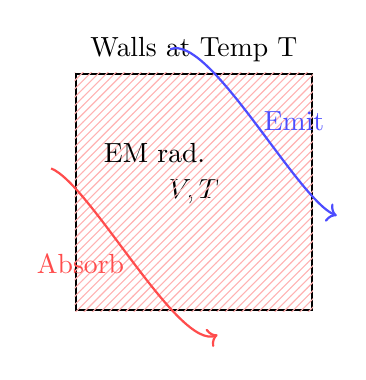
\begin{tikzpicture}
    \node (Box) [draw, thick, minimum width=3cm, minimum height=3cm, label=center:{$V, T$}] {};
    \fill [pattern=north east lines, pattern color=red!30] (Box.south west) rectangle (Box.north east);
    \node at ($(Box.north)+(0,0.3)$) {Walls at Temp T};
    \node at ($(Box.center) + (-0.5,0.5)$) {EM rad.};
    \draw[->, thick, red!70] ($(Box.west)+(-0.3,0.3)$) .. controls +(0.5,-0.2) and +(-0.5,-0.2) .. ($(Box.south)+(0.3,-0.3)$) node[pos=0.5, left] {Absorb};
    \draw[<-, thick, blue!70] ($(Box.east)+(0.3,-0.3)$) .. controls +(-0.5,0.2) and +(0.5,0.2) .. ($(Box.north)+(-0.3,0.3)$) node[pos=0.5, right] {Emit};
\end{tikzpicture}
\end{center}
The walls continually absorb \& emit radiation. In equilibrium, the properties of the EM radiation depend only on $T$.

Wave-particle duality of QM $\implies$ EM radiation can be described as waves (classical EM) or particles ("photons").
\begin{itemize}
    \item Photons are bosons.
    \item Photon number is not conserved (can be absorbed/emitted by walls).
    \item Interactions between photons are negligible (because Maxwell's equations are linear).
\end{itemize}
Therefore, we may treat the equilibrium EM radiation as an ideal gas of photons obeying photon statistics ($\mu=0$).

\subsection*{Single-Particle States for Photons}

Need to specify the states $r$ and energies $\eps_r$.
From Maxwell's equations in vacuum, the electric field $\vec{E}$ satisfies the wave equation:
\[ \nabla^2 \vec{E} = \frac{1}{c^2} \pderiv[2]{\vec{E}}{t^2} \]
Plane wave solutions $\vec{E} = \text{Re}\{\vec{E}_0 e^{i(\vec{k}\cdot\vec{x} - \omega t)}\}$ require the dispersion relation $\omega = c |\vec{k}| = ck$.
Also, $\nabla \cdot \vec{E} = 0 \implies \vec{k} \cdot \vec{E}_0 = 0$, so $\vec{E}$ is transverse to $\vec{k}$. For each $\vec{k}$, there are two linearly independent modes of oscillation (polarization states) perpendicular to $\vec{k}$.

In the particle description (QM):
\begin{itemize}
    \item Photon energy: $\eps = \hbar\omega = \hbar c k$.
    \item Photon momentum: $\vec{p} = \hbar\vec{k}$.
    \item Energy-momentum relation: $\eps = c |\vec{p}| = cp$. (Massless particle).
\end{itemize}
A single-photon state $r$ is specified by its wave-vector $\vec{k}$ (or momentum $\vec{p}$) and its polarization state $s$ (two possibilities, $s=1, 2$).
The energy $\eps_k = \hbar c k$ is independent of polarization.

\subsection*{Photon Gas Thermodynamics}

The mean number of photons in a state $(\vec{k}, s)$ is given by the Planck distribution ($\mu=0$):
\[ \nbar_{\vec{k}, s} = \frac{1}{e^{\beta \eps_k} - 1} = \frac{1}{e^{\beta \hbar c k} - 1} \]

\textbf{Counting States:}
Use Periodic Boundary Conditions (PBC) on a large box $V=L_x L_y L_z$.
Allowed wave-vectors: $k_i = 2\pi n_i / L_i$.
Sum over states $\sum_r$ becomes sum over $(\vec{k}, s)$. Spin degeneracy $g=2$ for polarization.
\[ \sum_r \to \sum_{\vec{k}, s=1,2} \to g V \int \frac{d^3k}{(2\pi)^3} = 2V \int \frac{d^3k}{(2\pi)^3} \]
Convert integral to frequency $\omega = ck$. Use spherical coordinates in k-space ($d^3k = 4\pi k^2 dk$).
\[ \sum_r \to 2V \int_0^\infty \frac{4\pi k^2 dk}{(2\pi)^3} = \frac{V}{\pi^2} \int_0^\infty k^2 dk \]
Since $k=\omega/c$, $dk=d\omega/c$:
\[ \sum_r \to \frac{V}{\pi^2} \int_0^\infty \left(\frac{\omega}{c}\right)^2 \left(\frac{d\omega}{c}\right) = \int_0^\infty d\omega \left( \frac{V \omega^2}{\pi^2 c^3} \right) \]
We define the density of modes (states) per unit frequency range $g(\omega)$:
\[ g(\omega) d\omega = \frac{V \omega^2}{\pi^2 c^3} d\omega \]
\[ g(\omega) = \frac{V \omega^2}{\pi^2 c^3} \]

\subsection*{Planck's Formula}

Use this result to investigate the mean energy of the photon gas.
\[ E = \sum_r \nbar_r \eps_r = \int_0^\infty d\omega \, g(\omega) \nbar(\omega) \eps(\omega) \]
where $\nbar(\omega) = 1/(e^{\beta\hbar\omega}-1)$ and $\eps(\omega) = \hbar\omega$.
\[ E = \int_0^\infty d\omega \left( \frac{V \omega^2}{\pi^2 c^3} \right) \left( \frac{1}{e^{\beta\hbar\omega} - 1} \right) (\hbar\omega) \]
\[ E = \frac{V \hbar}{\pi^2 c^3} \int_0^\infty d\omega \frac{\omega^3}{e^{\beta\hbar\omega} - 1} \]
Write this as $E = \int_0^\infty d\omega (\frac{dE}{d\omega})$. The spectral energy density (mean energy per unit volume per unit frequency range) is $u(\omega) = \frac{1}{V} \frac{dE}{d\omega}$.
\[ u(\omega) = \frac{\hbar}{\pi^2 c^3} \frac{\omega^3}{e^{\beta\hbar\omega} - 1} \]
This is \textbf{Planck's formula} for black-body radiation.

Plot $u(\omega)$ vs $\omega$. It is useful to use a dimensionless variable $x = \beta\hbar\omega = \hbar\omega/T$. $\omega = Tx/\hbar$, $d\omega = Tdx/\hbar$.
\[ u(\omega) d\omega = \frac{\hbar}{\pi^2 c^3} \frac{(Tx/\hbar)^3}{e^x - 1} \left(\frac{T}{\hbar} dx\right) = \frac{T^4}{\pi^2 (\hbar c)^3} \frac{x^3}{e^x - 1} dx \]
Let $f(x) = \frac{x^3}{e^x-1}$.

\begin{center}
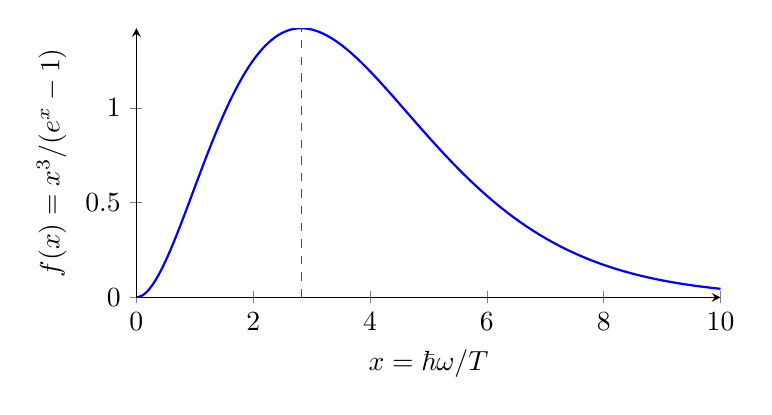
\begin{tikzpicture}
\begin{axis}[
    xlabel={$x = \hbar\omega/T$}, ylabel={$f(x) = x^3 / (e^x-1)$},
    xmin=0, ymin=0,
    axis lines=left,
    samples=101, smooth, domain=0.01:10,
    width=9cm, height=5cm
]
\addplot [thick, blue] {x^3 / (exp(x)-1)};
% Max value
\xdef\xmax{2.8214} % Approximate value where x^3/(e^x-1) is max
\pgfmathsetmacro{\ymax}{\xmax^3 / (exp(\xmax)-1)}
\draw [dashed, red] (axis cs:\xmax, 0) node[below] {$x_{max} \approx 2.821$} -- (axis cs:\xmax, \ymax);
\end{axis}
\end{tikzpicture}
\end{center}
The function $f(x)$ peaks at $x_{max} \approx 2.821$. This means the peak frequency $\omega_{max}$ in the spectrum satisfies $\hbar\omega_{max} / T \approx 2.821$.
\[ \hbar\omega_{max} \approx 2.821 T \quad \text{or} \quad \omega_{max} \approx \frac{2.821 T}{\hbar} \]
As $T$ increases, the maximum of the spectral distribution shifts to higher frequencies, proportional to $T$. This is \textbf{Wien's displacement law}.

\textbf{Low Frequency Limit ($\hbar\omega \ll T$, or $x \ll 1$):}
$e^x \approx 1+x$.
$u(\omega) \approx \frac{\hbar}{\pi^2 c^3} \frac{\omega^3}{(1+x)-1} = \frac{\hbar}{\pi^2 c^3} \frac{\omega^3}{x} = \frac{\hbar}{\pi^2 c^3} \frac{\omega^3}{\beta\hbar\omega} = \frac{T}{\pi^2 c^3} \omega^2$.
\[ u(\omega) \approx \frac{T \omega^2}{\pi^2 c^3} \quad (\text{Rayleigh-Jeans formula}) \]
This classical result follows from equipartition: each EM mode (oscillator) has average energy $T$. $T \times (\text{number of modes per frequency per volume})$ gives $T \times (\omega^2/(\pi^2 c^3))$.
Note: The temperature $T$ drops out of the average energy per mode $\avg{\eps} = \hbar\omega \nbar(\omega) \approx \hbar\omega / (\beta\hbar\omega) = T$, consistent with equipartition.

The RJ formula predicts $u(\omega) \propto \omega^2$, which diverges at high frequencies ($\omega \to \infty$). If integrated, it gives infinite total energy density. This is the \textbf{"ultraviolet catastrophe"} of classical physics. Planck's resolution was to introduce quantized energies $E=n\hbar\omega$, leading to the $e^{\beta\hbar\omega}-1$ denominator which suppresses high frequencies. This was a first success of quantum theory.

\subsection*{Total Energy Density (Stefan-Boltzmann Law)}

Compute the total energy density $u = E/V$.
\[ u = \int_0^\infty u(\omega) d\omega = \frac{T^4}{\pi^2 (\hbar c)^3} \int_0^\infty dx \frac{x^3}{e^x - 1} \]
The definite integral is $\int_0^\infty \frac{x^3}{e^x-1} dx = \Gamma(4)\zeta(4) = 3! (\pi^4/90) = 6\pi^4/90 = \pi^4/15$.
\[ u = \frac{T^4}{\pi^2 (\hbar c)^3} \frac{\pi^4}{15} = \frac{\pi^2}{15 (\hbar c)^3} T^4 \]
Energy density $u \propto T^4$. This is the \textbf{Stefan-Boltzmann Law}.
$u = \sigma_E T^4$, where $\sigma_E = \frac{\pi^2}{15 (\hbar c)^3}$. (If using $T$ in Kelvin, $\sigma_E = \frac{\pi^2 \kb^4}{15 \hbar^3 c^3}$).

Qualitatively: Each thermally relevant photon mode has energy $\sim T$. The relevant modes are those with $\hbar\omega \sim T$, or $\hbar c k \sim T$, so $k \lesssim k_{max} \sim T/(\hbar c)$. The number of modes per volume up to $k_{max}$ is $\sim k_{max}^3 \sim (T/(\hbar c))^3 \propto T^3$.
Total energy density $u \sim (\text{\# modes / vol}) \times (\text{avg energy per mode}) \propto T^3 \times T = T^4$.

\end{document}